%
%                       This is a basic LaTeX Template
%                       for the Informatics Research Review

\documentclass[a4paper,11pt]{article}
% Add local fullpage and head macros
\usepackage{head,fullpage}     
% Add graphicx package with pdf flag (must use pdflatex)
\usepackage[pdftex]{graphicx}  
% Better support for URLs
\usepackage{url}
% Date formating
\usepackage{datetime}

\newdateformat{monthyeardate}{%
  \monthname[\THEMONTH] \THEYEAR}

\parindent=0pt          %  Switch off indent of paragraphs 
\parskip=5pt            %  Put 5pt between each paragraph  
\Urlmuskip=0mu plus 1mu %  Better line breaks for URLs


%                       This section generates a title page
%                       Edit only the following three lines
%                       providing your exam number, 
%                       the general field of study you are considering
%                       for your review, and name of IRR tutor

\newcommand{\examnumber}{s2517285}
\newcommand{\field}{Edge Computing Offloading in Internet of Things: Experimental Designs and Configurations}
\newcommand{\supervisor}{My IRR Tutor}

\begin{document}
\begin{minipage}[b]{110mm}
        {\Huge\bf School of Informatics
        \vspace*{17mm}}
\end{minipage}
\hfill
\begin{minipage}[t]{40mm}               
        \makebox[40mm]{
        
\includegraphics[width=40mm]{crest.png}}
\end{minipage}
\par\noindent
    % Centre Title, and name
\vspace*{2cm}
\begin{center}
        \Large\bf Informatics Research Review \\
        \Large\bf \field
\end{center}
\vspace*{1.5cm}
\begin{center}
        \bf \examnumber\\
        \monthyeardate\today
\end{center}
\vspace*{5mm}

%
%                       Insert your abstract HERE
%                       
\begin{abstract}
        The abstract is a short concise outline of your 
        project area, {\bf of no more than 100 words}.
\end{abstract}

\vspace*{1cm}

\vspace*{3cm}
Date: \today

\vfill
{\bf Supervisor:} \supervisor
\newpage

%                                               Through page and setup 
%                                               fancy headings
\setcounter{page}{1}                            % Set page number to 1
\footruleheight{1pt}
\headruleheight{1pt}
\lfoot{\small School of Informatics}
\lhead{Informatics Research Review}
\rhead{- \thepage}
\cfoot{}
\rfoot{Date: \date{\today}}
%

\section{Introduction}

%物联网的发展
Internet of Things (IoT) means that the objects around people can communicate with each other and cooperate to achieve common goals, which has great potential for both private and business uses \cite{iot}. Most tasks handled by devices in IoT tend to be delay-sensitive, which also generate an amount of data of nearly 49 EB \cite{Distributed_Offloading_in_Overlapping_Areas}. However, the IoT devices are usually limited in terms of memory, battery life, and computing power \cite{Internet_of_Things_offloading_Ongoing_issues, A_Cooperative_Partial_Computation_Offloading_Scheme_for_Mobile_Edge}. Hence, it is impossible to process all the application tasks in local devices and meanwhile satisfy all the performance requirements \cite{Distributed_Offloading_in_Overlapping_Areas}. As a consequence, computation offloading is applied to solve this problem. Computation offloading means the tasks on the user equipment (IoT devices) can be transmitted to the remote server while getting the result after the remote server has successfully processed the tasks \cite{offloading_strategy}. Hence, the local devices are not required to be equipped with advanced hardware or software which could be expensive. \newline\newline
In tradition, cloud computation integrates with the Internet of Things since cloud server has great capability. Unlike IoT, the storage and computation power provided centrally by the cloud server is almost unlimited, which corresponds to the disadvantages of IoT \cite{cloud_advatange,cloud_central}. Hence, cloud computing can help IoT devices to complete their computation tasks with high performance. However, for IoT devices, it is an obstacle to obtaining stable and acceptable network performance to reach the cloud \cite{cloud_advatange_and_problem}. Additionally, the cloud server has to be challenged by reliability problems since the devices may fail or become inaccessible \cite{cloud_advatange_and_problem}. Unfortunately, the extensive scale of the resultant system, stemming from interactions with a significant number of devices, renders the rising requirements for storage capacity and computational power in subsequent processing progressively difficult to meet \cite{cloud_advatange_and_problem}. Therefore, edge computing is introduced to address the issues of the IoT and the cloud. \newline\newline
Edge Computing (EC), also named Mobile Edge Computing (MEC), provides cloud computing capabilities within the Radio Access Network close to mobile users \cite{EC_definition}. Compared with cloud computing, edge computing is more likely to compute in real-time because the edge servers are located at places closer to the users \cite{edge_advantage_archetecture}. Moreover, edge computing doesn't need the users to upload the data to the cloud computing center and reduce the load on the network bandwidth, which lowers the cost and the network bandwidth pressure \cite{edge_advantage_archetecture}. Many algorithms have been designed to optimize the task offloading problem in IoT applications based on edge computing. Nevertheless, these algorithms shown high performance have not been systematically compared to come to a conclusion about the best algorithm. One of the reasons is the experimental designs and configurations for each algorithm are extremely different. For example, one configuration includes the cloud component while another only considers the edge servers. Consequently, it is difficult to get an objective comparison. \newline\newline
As edge computing plays a more and more significant role in coordinating the work between IoT devices, it is necessary to design optimization algorithms to enhance the functionality of IoT through the utilization of Edge Computing characteristics. Quantities of optimization algorithms have been proposed and implemented, however, it is impossible to compare their performance due to the difference between system models (edge computing models). There are several important components that can be used to build different kinds of edge computing models for IoT devices, which may have a great impact on the performance of the algorithms on edge computing. Hence, this review will summarize the designs or configurations for the IoT application based on edge computing. It is noted that the pattern mentioned only includes the cloud server, edge server and objective function.\newline\newline
To address the problem of differences in edge computing system models that result in incomparability, this article will attempt to answer the following questions:
        \begin{quote}
                1. What are the main differences between different system models? How do those affect the performance of the algorithms?
        \end{quote}
        \begin{quote}
                2. Why did the designers choose such configurations? What are the pros and cons?
        \end{quote}
        \begin{quote}
                3. Based on questions 1 and 2, what designs or configurations should be considered when applying optimization algorithms?
        \end{quote}
\noindent Section 2 will focus on the cloud computing component in the EC designs. Additionally, in section 3 the full offloading and partial offloading will be discussed. Last but not least, section 4 will study the different objective functions chosen by the EC system models.
        

% and attempt to classify the models by finding similar configurations across the models. It should be noted that the pattern mentioned only including cloud server, edge server and objective function. For the similar models, their difference also will be discussed in the review. Additionally, the second question answered is the reason why these papers design such models and what is the benefit of the models. Furthermore, based on the results above, the review will try to derive a conclusion: What model should be employed for the implementation and comparison of existing algorithms.



% 许多算法被应用,但是他们的实验配置不同,难以比较

% 本文对不同的实验配置进行总结和介绍(架构不同、设备的不同),为什么他们要选择这样的配置,并尝试找出几种模式

% 1. 系统和问题的模型有哪些?他们是否有相似的模式,以及这些相似的模式中的每个模型的不同之处
% 2. 为什么要选这样的模型?这样的模式有什么好处
% 3. 基于1和2,找出应该使用什么模型来实现和比较已有的算法

%cloud server, edge computing and cost function
\section{Literature Review}
\subsection{Cloud Computing components}
Though the main conception discussed in this review is edge computing, it doesn't mean that the cloud components should be excluded from the edge computing models. Because edge computing and cloud computing are not mutually exclusive, instead they are complementary. However, there exist some papers which don't agree to include the cloud components for some reasons.\newline




Zhang et.al has constructed a model which doesn't consider the cloud server in the system model. They suggest that transmission failure probability can be largely reduced if the tasks aren't offloaded to the cloud server. Additionally, they believe that the model has to suffer from significant delay if introducing the cloud server, while the quality of experience can be guaranteed by their designed cooperative network. It should be noted that each edge server only belongs to one cooperative network based on the physical distance and the cluster of the edge servers will be divided into \textit{K} cooperative networks. Furthermore, the IoT device will offload the tasks to the closest edge server. Nevertheless, since the model also adds constraints to the edge servers on the maximum throughput of processing the tasks, the cooperative will assist in redirecting the offloaded task to other nearby edge servers \cite{no_cloud_1_density}. Additionally, Ali et.al attempts to concentrate on the smart offloading of IoT devices for edge computing, hence the cloud computing component is unnecessary for the algorithm research \cite{granuity_2}.\newline % 找找看还有没有其他不包括云的

Nevertheless, When the number of tasks doesn't exceed a threshold based on the number of edge servers, the edge servers can provide better service due to the shorter transfer time. However, if the number of tasks grows beyond the threshold, the shortage of the computation resources of the edge servers compared to the cloud server will show the impact on performance \cite{A_Cooperative_Partial_Computation_Offloading_Scheme_for_Mobile_Edge}. Hence, it is reasonable to introduce the cloud server, with powerful computing resources and computing power, to help take the burden of the edge servers by processing an excessive number of tasks. Nonetheless, for those models that have included the cloud server, there is a problem with how to coordinate the edge servers and the cloud server's tasks. \newline

Ning et.al has proposed a computation offloading model that the IoT equipment that sends offloading requests to the small evolved NodeBs (SeNBs), while SeNBs take the responsibility of offloading tasks to the edge server or the cloud server according to schedule algorithms \cite{A_Cooperative_Partial_Computation_Offloading_Scheme_for_Mobile_Edge}. This model also supposes that the transmission delay between SeNBs and edge servers can be ignored \cite{A_Cooperative_Partial_Computation_Offloading_Scheme_for_Mobile_Edge}, which means sending tasks to the edge server or cloud server via SeNBs takes the same amount of time as sending it directly to the edge or cloud server. To better simulate the characteristics of the edge servers and cloud servers, the model adds constraints to the number of tasks to be processed for every edge server, but cloud servers have no such constraints \cite{A_Cooperative_Partial_Computation_Offloading_Scheme_for_Mobile_Edge}. Additionally, a similar model designed by Jiang et.al sets a manager in edge computing servers to decide where to process the tasks according to the result of the optimization algorithm. The role of the manager is similar to the SeNBs, but the manager is responsible for the whole assignment of tasks, rather than the assignment of offloaded tasks \cite{cloud_3_edgemanager}. These models set a special model to gather the edge servers and cloud server real-time information \cite{A_Cooperative_Partial_Computation_Offloading_Scheme_for_Mobile_Edge}. Hence, the extra transmission delay can be avoided since the IoT devices are not required to get the information of servers' available resources. \newline

\begin{figure}[h]
        \centering
        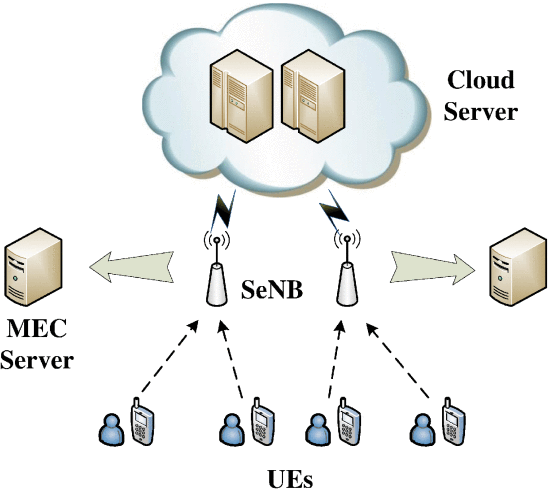
\includegraphics[width=0.5\textwidth]{SeNBs.png}
        \caption{Special server to schedule \cite{A_Cooperative_Partial_Computation_Offloading_Scheme_for_Mobile_Edge}}
\end{figure}

Another computation model created by Chen et.al also includes cloud computing components, however, the architecture differentiates from Ning's model. The SeNBs are used to schedule whether the task offloading request is sent to the edge server or cloud server in Ning's model. However, in Chen's model, all offloaded tasks are sent to the edge server at first, if the edge server can't process more tasks, some tasks will be offloaded to the cloud server to reduce the burden of the edge server \cite{cloud_2_edgeconnectedtocloud}. Hence, this model has to judge by itself whether it can process the coming tasks 

\begin{figure}[h]
        \centering
        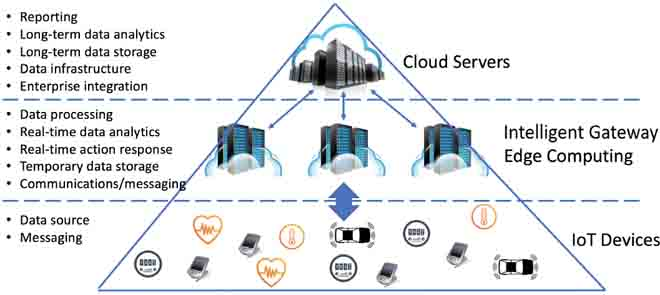
\includegraphics[width=0.5\textwidth]{edgeconnectedcloud.jpg}
        \caption{Offloading tasks directly from edge server to cloud server \cite{aim_offloading}}
\end{figure}
\newpage
Hence, whether the cloud computing component is included can have a great impact on the system model since there are pros and cons to using cloud servers. The cloud server can provide a huge amount of computing resources. However, due to the distance from IoT devices to the cloud, the delay or the energy consumption has to be considered which could increase the complexity of the model and has the potential to lower the performance. Furthermore, the role of deciding the direction of the offloading tasks is significant, in light of the fact that different roles would select different strategies. 


% --什么时候选择有云服务器
% --云服务器的作用
% 使用云服务器后模型发生了什么变化
% --A是如何把EC和CC结合起来的(或者不结合CC),B是如何结合起来的,C是如何结合起来的,每次论述的时候加上这篇文章不同的地方以及为什么这么不同
% --什么时候把任务卸载到云服务器
% 总结:当前比较流行的是传统的云计算,现在的模式是边缘计算处理一些,再让云计算处理一些 \cite{why_cloud}. 但是考虑云计算的话模型会变得更复杂,模型需要考虑什么时候,把什么任务,由谁交给云计算处理,因此,如果只是研究edge computing的算法的话,不考虑云计算比较好;但如果更考虑现实的应用的话,需要考虑云计算

\subsection{Offloading Strategies}
Since IoT devices have limited computation and energy resources, they can hardly satisfy the complicated tasks required by the IoT service. Therefore, the goal of the task offloading is to gain computation capability without using more energy-cost devices \cite{aim_offloading}. The offloading strategies can be separated into two categories: full offloading and partial offloading strategies. A full offloading strategy means offloading the task all to the edge computing server or cloud server. On the contrary, the partial offloading strategy is aimed at dividing tasks into several parts, one part is executed on the local machine while the other parts are offloaded to the edge server or cloud server \cite{full_partial}. 

\begin{figure}[h]
        \centering
        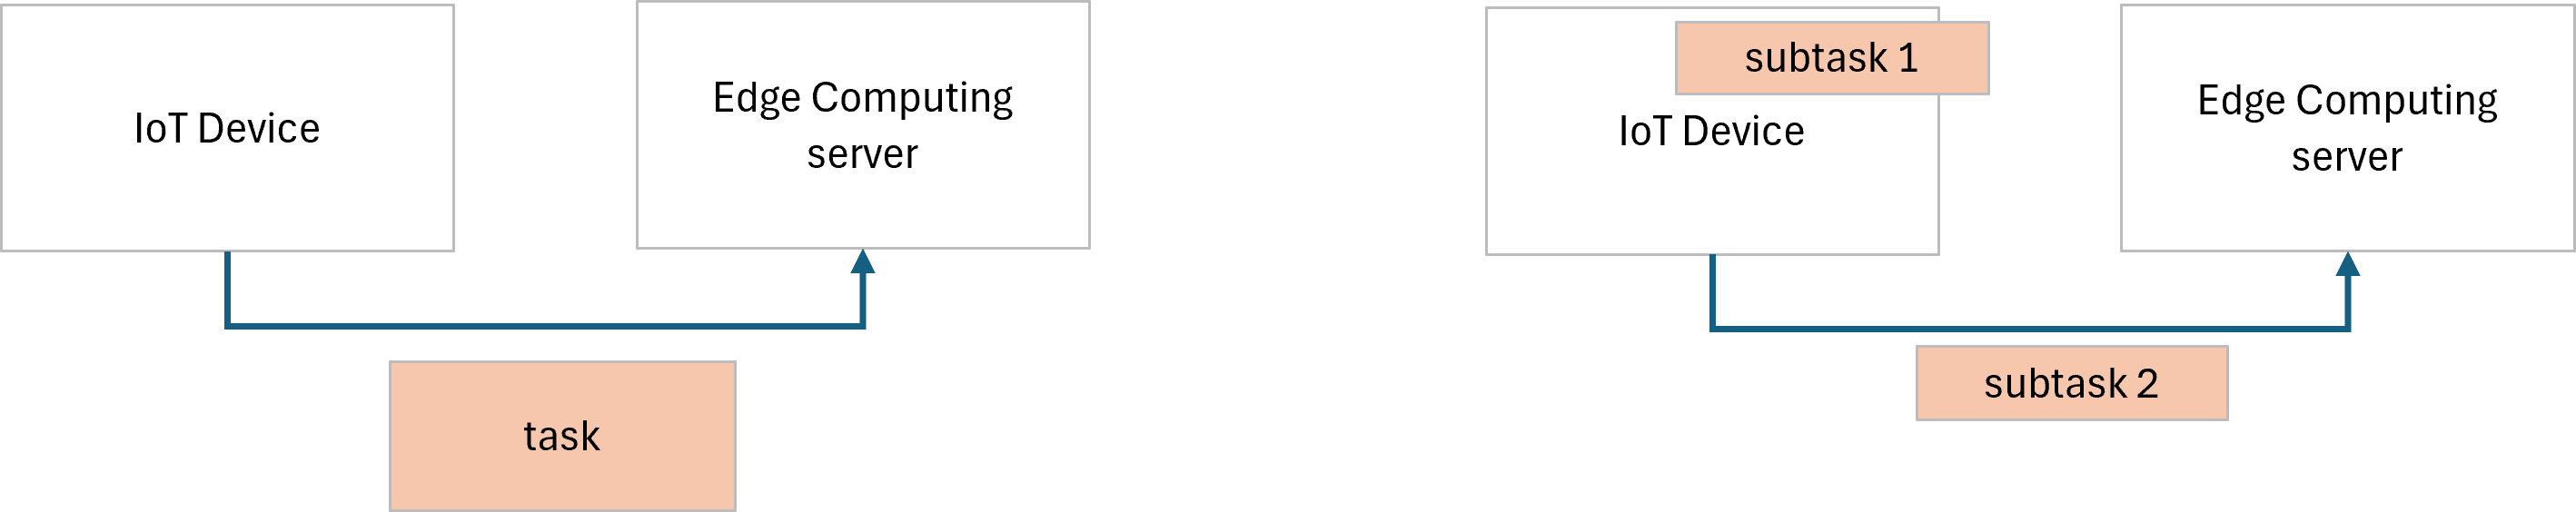
\includegraphics[width=0.8\textwidth]{offloading.png}
        \caption{Full offloading strategy VS partial offloading strategy}
\end{figure}

Zhang et.al applies a full offloading strategy to process the tasks, unlike the partial offloading strategy, which treats the task as the smallest unit \cite{no_cloud_1_density}. Another research proposed by Chen et.al also chooses full offloading strategies \cite{full_offload_2}. The reason that they both make such a choice is that from their point of view, due to the heterogeneity of the IoT devices, it is unlikely to gather the prior statistical information such as the size of the coming tasks \cite{no_cloud_1_density,full_offload_2}. Hence, from this perspective, the better option is the full offloading strategy since it makes the model more general and realistic. %In addition, another article's option is also full offloading because \cite{cloud_2_edgeconnectedtocloud}
\newline\newline
However, Ning et.al supports the partial offloading strategy rather than the full offloading strategy. They suggest that one factor that affects the choice of different strategies is the type of applications. For example, if the input data of the application is private information, the tasks should be partially offloaded. Nevertheless, the complex relationships between different modules in each task can make the model become more complicated. Therefore, to simplify the model, the complicated module dependency system (the module refers to the part of the tasks) has been simplified into a linear sequence processing module which means the output of the last module is the input of the next module. Moreover, the paper emphasizes that the computation offloading model can be applied to the tasks that are not allowed to be offloaded, since the module has a flag to indicate whether the module is executed locally or remotely in edge or cloud server \cite{A_Cooperative_Partial_Computation_Offloading_Scheme_for_Mobile_Edge}. As a result, their offloading model becomes more general since it not only can capture the situation of full and partial offloading but also can capture the case where the task is executed locally on IoT devices.
\newline\newline
There are many other factors that affect the offload strategy, such as the quality of communication links, the computing resource availability of the cloud and edge server, and IoT devices's abilities \cite{A_Cooperative_Partial_Computation_Offloading_Scheme_for_Mobile_Edge}. Furthermore, based on the condition that the task is allowed to be divided, for the reason of optimizing the user's energy conservation, partial offloading strategy has a higher priority \cite{save_energy}. However, the offloading becomes more complicated when the partial offloading strategy is considered, for the reason that the task relevance, characteristics and segmentation have to be concentrated \cite{user_central}. \newline

It is worth mentioning that even though those experiments choose partial offloading strategies, there is a big difference in the level of granularity they use when dividing tasks into subtasks. Huang et.al's partial offloading strategy considers the tasks that can be partitioned at any granularity. Consequently, the optimization problem of this model becomes non-linear and non-convex, which is more challenging to solve \cite{Distributed_Offloading_in_Overlapping_Areas}. By contrast, since Ning's model only considers the linear sequence relationship, the model is simpler to solve as a mixed integer linear problem \cite{A_Cooperative_Partial_Computation_Offloading_Scheme_for_Mobile_Edge}. Nevertheless, Ali et.al has proposed a more systematic way to partition the tasks. Instead of fixing the number of modules or allowing partition of arbitrary granularity, they apply deep neural networks (DNN) to find the optimal components and the optimal way to partition. The dataset, consisting of the size of the task, the minimum size of the module or partition, the largest possible number of components and other information, will be generated by a comprehensive cost function \cite{granuity_2}. As a consequence, after training the model, it can generate a partition policy for the coming tasks.\newline

As discussed above, the heterogeneity of the edge server, the unknown upcoming tasks, and the difficulty of reasonably dividing the tasks make the full offloading strategy more appealing. However, some specific information hidden in the tasks, the energy-saving requirements and other factors give support to the application of the partial offloading strategy. 
% xx文章选择了哪种卸载,具体如何建模的,以及选择这种卸载的理由
% 部分卸载有什么优点、缺点
% 怎么划分子任务,将子任务部分卸载
% 1.假设所有任务可以无限度划分\cite{Distributed_Offloading_in_Overlapping_Areas}
% 卸载的第二种分类:如何卸载到多个edge server,什么时候卸载到云服务器(从用户还是从edge server)
% 使用完全卸载/部分卸载后,模型发生了什么变化(or 计算发生了什么变化)
% 总结

\subsection{Objective Functions}
The objective function can be composed of one or several objectives. Hence, if one objective function focuses on delay, and another objective function focuses on energy, it is hard to compare the performance of the optimization algorithms since they optimize in different directions. Hence, it is essential to review different objective functions in previous literatures.\newline

The objective function chosen by Ning et.al focused on computation offloading delay which consists of process time and transmission time \cite{A_Cooperative_Partial_Computation_Offloading_Scheme_for_Mobile_Edge}. It should be noted that the subject of the objective function is the module (the partition of the tasks). Hence, whether the module is executed locally or remotely on an edge server or cloud server can have an impact on the process and transmission delay. To conclude, the objective function only focuses on the total delay of the tasks. Additionally, the objective function of another model also concentrated on the delay. However, it is significant that for both of the objective functions, different edge server has different computing capabilities.  \cite{no_cloud_1_density}. For example, the edge server in Ning's model can only process one offloading request at a time, but another objective function uses the maximum size of total tasks to constrain the objective function, which means the edge server can process multiple tasks at the same time. Moreover, the subjects involved in the model are distinct, one pertains to the module, while the other corresponds to the task itself. \newline

Instead of concentrating on the delay, the model created by Chen et.al has used a cost function to replace the total delay. This cost function consists of network cost and transmission cost, which can be influenced by the number of offloaded tasks, the traffic and other factors \cite{full_offload_2}. Hence, this objective function is based on the actual cost of using the network, edge server and cloud server. Although it takes into account delay, it is merely considered as a constraint rather than an optimization objective. As a consequence, comparing the optimal solution of the algorithm with the optimal solution of the previous models' solution is meaningless.\newline

Except for the delay and the cost, objective functions can also be dominated by energy. According to the study conducted by Fu et.al, the objective function cares about the energy consumption caused by task processing and task offloading. Moreover, the delay and the limitation of the computation resources are constraints on the objective function \cite{objective_energy_2}. Hence, the definition of the optimal solution could be slightly different from the delay or the cost objective functions. \newline

Lu et.al's model is different from others since IoT devices are equipped with energy storage equipment and energy collector. As a consequence, the objective function is restricted by the power stored in the storage equipment. Furthermore, the function consists of three different objectives: service delay, energy consumption and task success rate based on coding error probability which hasn't been discussed in other objective functions. The reason for considering the task success rate is that it is likely that when the downloading process results from the remote server, errors could happen during this process 
\cite{energy_objective}. Therefore, this objective function places a great emphasis on the quality of the service instead of only the delay or the cost. An objective function that is slightly different from the previous one consists of three objectives: delay, energy consumption and price. The aim of applying this objective function is to guarantee the quality of the service while lowering the energy consumption and the cost \cite{user_central}. \newline

In conclusion, the objective functions encompass various types, and each type of objective function has numerous variants. The emphasis of those objective functions is different, which makes the comparison between different types of optimization algorithms impossible. For example, the objective function composed of multiple objectives is more comprehensive and realistic at the cost of simplicity. 





% 有哪些objective functions
% 为什么选择这个objective functions
% 哪个更好,或者在比较的时候要选择哪个更加普遍性的objective function
% 模型发生了什么变化 or 计算发生了什么变化
% 总结
\subsection{Other Difference}
% 其他的不同


\section{Summary \& Conclusion}
This review has studied many kinds of literature on different edge computing optimization designs and configurations. One of the conclusions that can be drawn is that the main difference between different designs or configurations is the cloud computing component, offloading strategies and the objective function. \newline

For cloud computing component, 
% 在研究了大量的文献后,我们找到了
        %1. 在设计对edge computing的优化算法时,它们这些的实验和配置的主要不同:3个
        %2. 为什么会有这些不同,分别有哪些好处
        %3. 我们可以得出哪些配置或设计更适合用来应用优化算法

\section{Future Work}
% 还有很多的不同需要被考虑
% 基于这样的设计重新将已有的算法整合进来,并进行比较

%                Now build the reference list
\bibliographystyle{unsrt}   % The reference style
%                This is plain and unsorted, so in the order
%                they appear in the document.


\small
\bibliography{main}       % bib file(s).

\end{document}

